\documentclass{article}
\usepackage{amsmath}
\usepackage{tikz-cd}
\usetikzlibrary{matrix,positioning,calc,decorations.pathreplacing,arrows.meta}
\usepackage{algorithm}
\usepackage[noend]{algpseudocode}
\usepackage[margin=.75in]{geometry}
\makeatletter
\def\BState{\State\hskip-\ALG@thistlm}
\makeatother

\begin{document}
\section {Data Structure}
The algorithms noted here use the following data structures layout:

% Approach 1: TikZ for precise mapping arrows
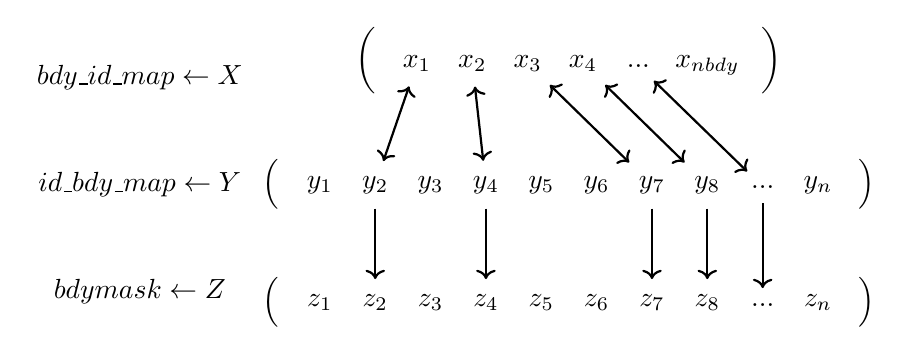
\begin{tikzpicture}[
    arr/.style={matrix of math nodes, left delimiter=(, right delimiter=), nodes={minimum width=2em}},
    map/.style={<->, shorten <=2pt, shorten >=2pt, thick},
    same/.style={->, shorten <=2pt, shorten >=2pt, thick}
]
    % Array A
    \matrix (A) [arr] {
        x_1 & x_2 & x_3 & x_4 & ... & x_{nbdy} \\
    };
    
    % Array B (shifted down)
    \matrix (B) [arr, below=8mm of A] {
        y_1 & y_2 & y_3 & y_4 & y_5 & y_6 & y_7 & y_8 & ... & y_n \\
    };

    % Array C (shifted down)
    \matrix (C) [arr, below=8mm of B] {
        z_1 & z_2 & z_3 & z_4 & z_5 & z_6 & z_7 & z_8 & ... & z_n \\
    };
    
    % Mapping arrows
    \draw[map] (A-1-1) -- (B-1-2);
    \draw[map] (A-1-2) -- (B-1-4);
    \draw[map] (A-1-3) -- (B-1-7);
    \draw[map] (A-1-4) -- (B-1-8);
    \draw[map] (A-1-5) -- (B-1-9);

    \draw[same] (B-1-2) -- (C-1-2);
    \draw[same] (B-1-4) -- (C-1-4);
    \draw[same] (B-1-7) -- (C-1-7);
    \draw[same] (B-1-8) -- (C-1-8);
    \draw[same] (B-1-9) -- (C-1-9);

    % Names
    \node[left=4mm of B] at (B.west) (bname) {$id\_bdy\_map \gets Y$} ;
    \node[above=8mm of bname] at (bname.north) (aname) {$bdy\_id\_map \gets X$} ;
    \node[below=8mm of bname] at (bname.south) (cname) {$bdymask \gets Z$} ;
\end{tikzpicture}

Where:
\begin{itemize}
    \item $bdy\_id\_map$ ($X$) contains $x_j$, whose value corresponds to an index $i$ into $id\_bdy\_map$ ($Y$)
    \item $id\_bdy\_map$ ($Y$) contains $y_i$, whose value corresponds to an index $j$ into $bdy\_id\_map$ ($X$)
    \item only $i$ indices of $bdymask$ ($Z$) with value $z_i > 0$ are mapped in $Y_i \leftrightarrow X_j$
    \item all other $i$ indices in $Y$ where $z_i \le 0 \rightarrow y_i = 0$
\end{itemize}

\section {Algorithms}
% First alg just gives us start, stop, nbdy, bdyIndex, idToIndex
\vspace{5mm}
\begin{algorithm}
\caption{Read the $mask\_dim$ in contiguous chunks, returning $start, stop, nbdy_{local}, X_{local}, Y_{local}$}\label{readbdymask}
\begin{algorithmic}[1]
\Function{read\_contiguous}{$domain$,$dims$,$global\_dim$,$mask\_dim$}
    \State
    \State $global\_size \gets get\_dim(global\_dim)$
    \State $start, stop \gets get\_index\_range(domain, global\_size)$
    \State $nread \gets stop - start$
    \State $io \gets open(get\_mesh\_stream(domain))$
    \State $read\_indices \gets [start, start+1, start+2, ..., start + nread]$
    \State
    \State $bdy\_indices \gets read(io, read\_indices, mask\_dim)$
    \State $nbdy_{local} \gets 0$
    \State $bdy\_map_{local} \gets [0_1, 0_2, ...0_{nread}]$
    \State $id\_map_{local} \gets [0_1, 0_2, ...0_{nread}]$
    \For {$i = 1, nread$}
        \If {$bdy\_indices[i] > 0$}
            \State $id\_map_{local}[i] \gets nbdy_{local}$
            \State $bdy\_map_{local}[nbdy_{local}] \gets i + start$
            \State $nbdy_{local} \gets nbdy_{local} + 1$
        \EndIf
    \EndFor

    \State $bdy\_map[:] \gets bdy\_map[:nbdy]$
    \State \Return $start, stop, nbdy, bdy\_map, id\_map$
\EndFunction
\end{algorithmic}
\end{algorithm}

\vspace{5mm}
\begin{algorithm}
\caption{Compute the $nbdy$ decomposition}\label{decomp}
\begin{algorithmic}[2]
\Function{bdy\_decomp}{$domain$,$block$,$global\_dim$,$mask\_dim$}
    \State
    \State $start, stop, nbdy_{local}, bdy\_map_{local}, id\_map_{local} \gets read\_contiguous(...)$
    \State $nproc \gets domain.nproc$
    \State $proc \gets domain.id$
    \State $nbdy(nproc) \gets \textbf{allgather($nbdy_{local}$)}$
    \State $nread(nproc) \gets \textbf{allgather($stop - start$)}$

    \State $csum_{nbdy} \gets csum_k = \sum_{i=1}^{k-1} nbdy_i$ where $k = 1 ... nproc$
    \State $csum_{nread} \gets csum_k = \sum_{i=1}^{k} nread_i$ where $k = 1 ... nproc$
    \State $id\_map_{local_{chunk}} \gets id\_map_{local}(:)$
    \State $bdy\_map_{local_{chunk}} \gets bdy\_map_{local}(:)$

    \State $bdymask_{block} \gets read(io, block.ownedIndices)$
    \State $reqbyproc_{block} \gets [0_1, 0_2, ..., 0_{nproc}]$
    \State $nreqindices_{block} \gets \textbf{list($nproc$)}$
    \State
    \State $j \gets 0$
    \For {$i = 1, block.nOwned$}
        \If {$bdymask_{block}[i] > 0$}
            \State $j \gets j + 1$
            \State $p \gets \textbf{findindex($csum_{nread} \ge block.indices[i]$)}$
            \State $nreqbyproc_{block}[p] \gets 1$
            \State $reqindices_{block}[p] \gets \textbf{add($block.indices[i]_{ij}$)}$
        \EndIf
    \EndFor
    \State
    \State $nreqbyproc_{global} \gets \textbf{allreduce($nreqbyproc_{block}$)}$
    \State
    \For {$iter, procid \in reqindices_{block}$}
        \If {$procid \ne proc$}
            \State \textbf{send($procid,$ all($iter$))}
        \EndIf
    \EndFor
    \State
    \State $reqindices_{global} \gets \textbf{list($nprocs$)}$
    \For {$i = 1, nreqbyproc_{global}[proc] - nreqbyproc_{block}[proc]$}
        \State $msg \gets \textbf{recv($anyproc, reqindices_p$)}$
        \State $reqindices_{global}[msg.proc] \gets \textbf{add($reqindices_p$)}$
    \EndFor
    \State
    \For {\textbf{each} $iter, procid \in reqindices_{global}$}
        \If {$procid \ne proc$}
            \State $indices \gets$ \textbf{list()}
            \For {$index \in iter$}
                \State $local\_index \gets id\_map_{local_{chunk}}[id - csum_{nread}[proc-1]]$
                \State $bdy_*= local\_index + csum_{nbdy}[proc]$
                \State $indices.add(bdy_*)$
            \EndFor
            \State \textbf{send($procid, indices$)}
        \EndIf
    \EndFor
    \State

    \For {\textbf{each} $iter, procid \in reqindices_{block}$}
        \If {$procid \ne proc$}
            \State $msg \gets \textbf{recv($procid, indices$)}$
            \For {$blockidx_{ij},recvidx_i \in \{iter,indices\}$}
                \State $i \impliedby blockidx_{ij}$
                \State $j \impliedby blockidx_{ij}$
                \State $id\_bdy\_map_{block}[i] \gets recvidx_i$
                \State $bdy\_id\_map_{block}[j] \gets blockidx_i$
            \EndFor
        \EndIf
    \EndFor
\EndFunction
\end{algorithmic}
\end{algorithm}

%%%%%%%%%%%%%%%%%%%%%%%%%%%%%%%%%%%%%%%%%%%%%%%%%%%%%%%%%%%%%%%%%%%%%%%%%%%%%%%%
% EXAMPLE START
%%%%%%%%%%%%%%%%%%%%%%%%%%%%%%%%%%%%%%%%%%%%%%%%%%%%%%%%%%%%%%%%%%%%%%%%%%%%%%%%
\newpage
\section {Example}
\subsection {Initial Setup} \label {setup}
Let us take the following $bdymask_{global}$ and $block$ assignments as an example:
\\\\
\vspace{5mm}
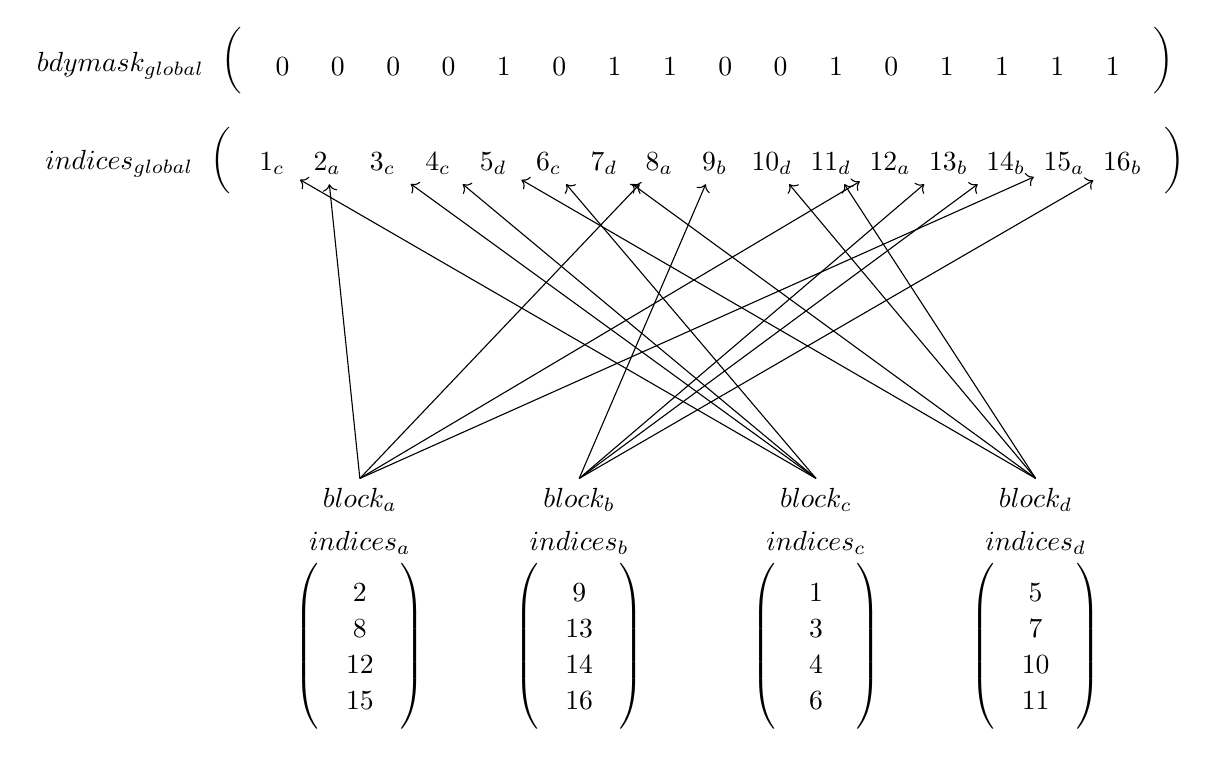
\begin{tikzpicture}[
    arr/.style={matrix of math nodes, left delimiter=(, right delimiter=), nodes={minimum width=2em}},
    map/.style={<->, shorten <=2pt, shorten >=2pt, thick},
    uni/.style={->}
]
    % Array C (shifted down)
    \matrix (C) [arr] {
    %   1   2   3   4   5   6   7   8   9  10  11  12  13  14  15  16
        0 & 0 & 0 & 0 & 1 & 0 & 1 & 1 & 0 & 0 & 1 & 0 & 1 & 1 & 1 & 1 \\
    };

    \matrix (D) [arr, below=5mm of C] {
        1_c & 2_a & 3_c & 4_c & 5_d & 6_c & 7_d & 8_a & 9_b & 10_d & 11_d & 12_a & 13_b & 14_b & 15_a & 16_b \\
    };

    % Names
    \node[left=4mm of C] at (C.west) (cname) {$bdymask_{global}$} ;
    \node[left=4mm of D] at (D.west) (dname) {$indices_{global}$} ;

    \node[below right=40mm and 10mm of D] at (D.west) (ablock) {$block_a$};
    \node[below right=40mm and 38mm of D] at (D.west) (bblock) {$block_b$};
    \node[below left=40mm and 38mm of D] at (D.east) (cblock) {$block_c$};
    \node[below left=40mm and 10mm of D] at (D.east) (dblock) {$block_d$};

    \node[below=0mm of ablock.south] (anode) {$indices_a$};
    \node[below=0mm of bblock.south] (bnode) {$indices_b$};
    \node[below=0mm of cblock.south] (cnode) {$indices_c$};
    \node[below=0mm of dblock.south] (dnode) {$indices_d$};

    
    \draw[uni] (ablock.north) -- (D-1-2);
    \draw[uni] (ablock.north) -- (D-1-8);
    \draw[uni] (ablock.north) -- (D-1-12);
    \draw[uni] (ablock.north) -- (D-1-15);
    
    \draw[uni] (bblock.north) -- (D-1-9);
    \draw[uni] (bblock.north) -- (D-1-13);
    \draw[uni] (bblock.north) -- (D-1-14);
    \draw[uni] (bblock.north) -- (D-1-16);
    
    \draw[uni] (cblock.north) -- (D-1-1);
    \draw[uni] (cblock.north) -- (D-1-3);
    \draw[uni] (cblock.north) -- (D-1-4);
    \draw[uni] (cblock.north) -- (D-1-6);

    \draw[uni] (dblock.north) -- (D-1-5);
    \draw[uni] (dblock.north) -- (D-1-7);
    \draw[uni] (dblock.north) -- (D-1-10);
    \draw[uni] (dblock.north) -- (D-1-11);

    \matrix (arra) [arr, below=0mm of anode.south] {
        2 \\ 8 \\ 12 \\ 15 \\
    };
    \matrix (arrb) [arr, below=0mm of bnode.south] {
        9 \\ 13 \\ 14 \\ 16 \\
    };
    \matrix (arrc) [arr, below=0mm of cnode.south] {
        1 \\ 3 \\ 4 \\ 6 \\
    };
    \matrix (arrd) [arr, below=0mm of dnode.south] {
        5 \\ 7 \\ 10 \\ 11 \\
    };
\end{tikzpicture}


%%%%%%%%%%%%%%%%%%%%%%%%%%%%%%%%%%%%%%%%%%%%%%%%%%%%%%%%%%%%%%%%%%%%%%%%%%%%%%%%
% EXPECTED
%%%%%%%%%%%%%%%%%%%%%%%%%%%%%%%%%%%%%%%%%%%%%%%%%%%%%%%%%%%%%%%%%%%%%%%%%%%%%%%%
\subsection {Expected Outcome} \label {output}
Our final product $bdy\_indices$ for each $block$ should be:
\\\\
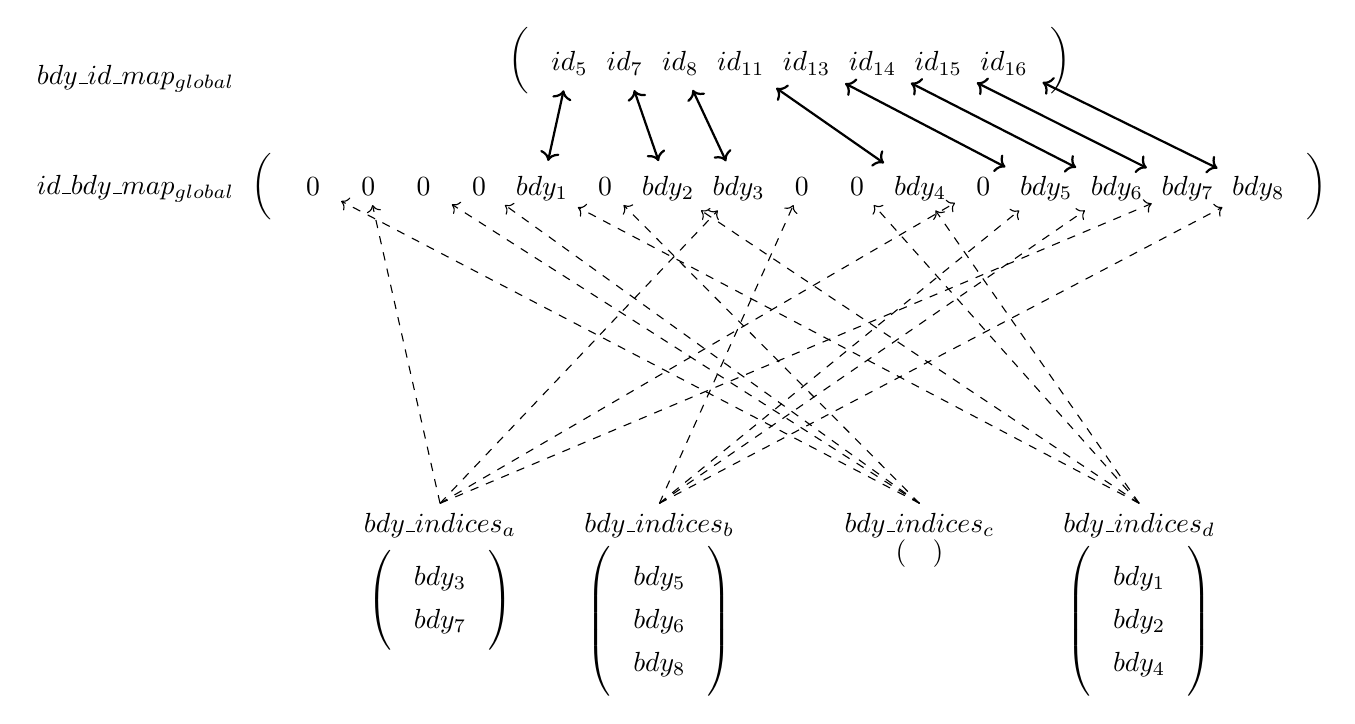
\begin{tikzpicture}[
    arr/.style={matrix of math nodes, left delimiter=(, right delimiter=), nodes={minimum width=2em}},
    map/.style={<->, shorten <=2pt, shorten >=2pt, thick},
    uni/.style={->}
]

    % Array A
    \matrix (A) [arr] {
        id_5 & id_7 & id_8 & id_{11} & id_{13} & id_{14} & id_{15} & id_{16} \\
    };

    % Array B
    \matrix (B) [arr, below=8mm of A] {
        0     & 0     & 0     & 0     &
        bdy_1 & 0     & bdy_2 & bdy_3 &
        0     & 0     & bdy_4 & 0     &
        bdy_5 & bdy_6 & bdy_7 & bdy_8 \\
    };

    \node[left=4mm of B] at (B.west) (bname) {$id\_bdy\_map_{global}$} ;
    \node[above=8mm of bname] at (bname.north) (aname) {$bdy\_id\_map_{global}$} ;

    % Mapping arrows
    \draw[map] (A-1-1) -- (B-1-5);
    \draw[map] (A-1-2) -- (B-1-7);
    \draw[map] (A-1-3) -- (B-1-8);
    \draw[map] (A-1-4) -- (B-1-11);
    \draw[map] (A-1-5) -- (B-1-13);
    \draw[map] (A-1-6) -- (B-1-14);
    \draw[map] (A-1-7) -- (B-1-15);
    \draw[map] (A-1-8) -- (B-1-16);


    \node[below right=40mm and 10mm of B] at (B.west) (anode) {$bdy\_indices_a$};
    \node[below right=40mm and 38mm of B] at (B.west) (bnode) {$bdy\_indices_b$};
    \node[below left=40mm and 38mm of B] at (B.east) (cnode) {$bdy\_indices_c$};
    \node[below left=40mm and 10mm of B] at (B.east) (dnode) {$bdy\_indices_d$};

    \matrix (arra) [arr, below=0mm of anode.south] {
        bdy_3 \\ bdy_7 \\
    };
    \matrix (arrb) [arr, below=0mm of bnode.south] {
        bdy_5 \\ bdy_6 \\ bdy_8 \\
    };
    \matrix (arrc) [arr, below=0mm of cnode.south] {
        \\
    };
    \matrix (arrd) [arr, below=0mm of dnode.south] {
        bdy_1 \\ bdy_2 \\ bdy_4 \\
    };
    
    % Mapping arrows
    \draw[uni, dashed] (anode.north) -- (B-1-2);
    \draw[uni, dashed] (anode.north) -- (B-1-8);
    \draw[uni, dashed] (anode.north) -- (B-1-12);
    \draw[uni, dashed] (anode.north) -- (B-1-15);
    
    \draw[uni, dashed] (bnode.north) -- (B-1-9);
    \draw[uni, dashed] (bnode.north) -- (B-1-13);
    \draw[uni, dashed] (bnode.north) -- (B-1-14);
    \draw[uni, dashed] (bnode.north) -- (B-1-16);
    
    \draw[uni, dashed] (cnode.north) -- (B-1-1);
    \draw[uni, dashed] (cnode.north) -- (B-1-3);
    \draw[uni, dashed] (cnode.north) -- (B-1-4);
    \draw[uni, dashed] (cnode.north) -- (B-1-6);
    
    \draw[uni, dashed] (dnode.north) -- (B-1-5);
    \draw[uni, dashed] (dnode.north) -- (B-1-7);
    \draw[uni, dashed] (dnode.north) -- (B-1-10);
    \draw[uni, dashed] (dnode.north) -- (B-1-11);

\end{tikzpicture}
\newpage
\subsection {Read Contiguous Data} \label {readdata}
Using the data above, and assuming the $blocks$ proceed in alphabetical order, using Algorithm~\ref{readbdymask} should yield
the following. The $..._{local_*}$ designation here pertains to contiguous chunk assignment, not $block$-specific.

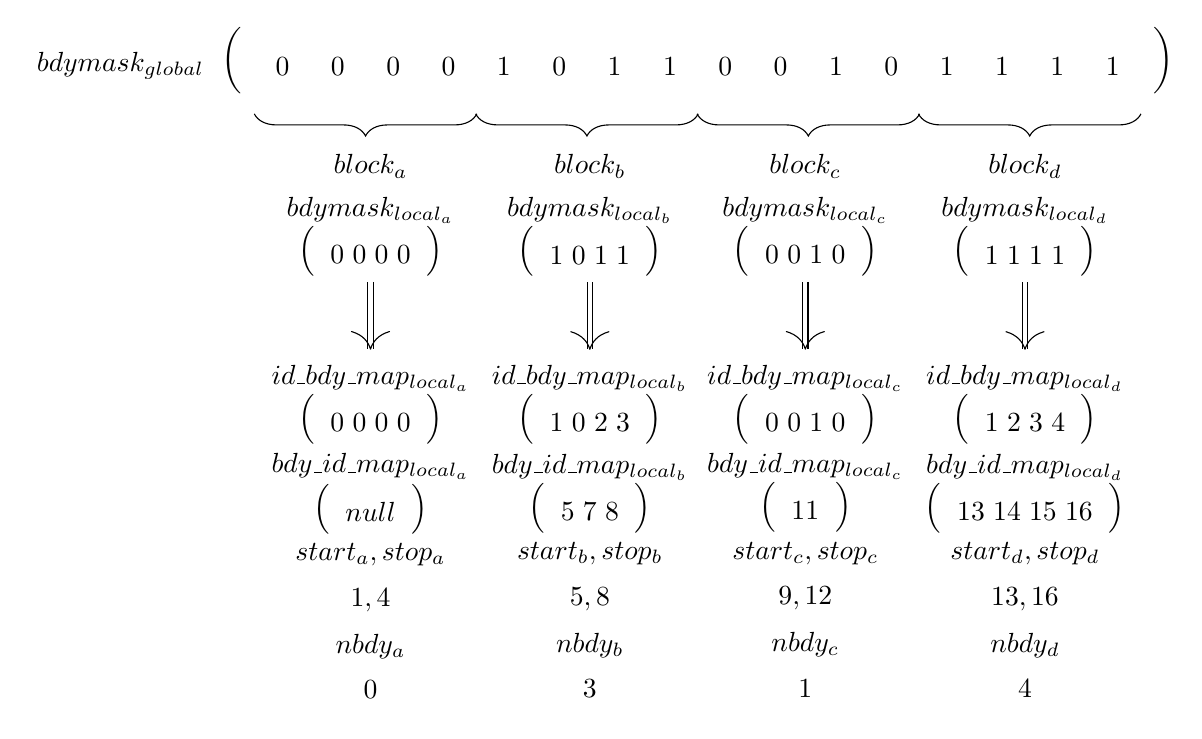
\begin{tikzpicture}[
    arr/.style={matrix of math nodes, left delimiter=(, right delimiter=), nodes={minimum width=2em}},
    smarr/.style={matrix of math nodes,
        % 1. Reduce space inside each cell (default is 0.333em)
        nodes={inner sep=1pt}, 
        % 2. Reduce space between rows and columns
        row sep=1pt,
        column sep=1pt,
        left delimiter=(, right delimiter=)},
    nopar/.style={matrix of math nodes, nodes={inner sep=1pt},row sep=1pt,column sep=1pt},
    map/.style={<->, shorten <=2pt, shorten >=2pt, thick},
    uni/.style={->},
    yield/.style={->,double,double equal sign distance,shorten <=2pt, shorten >=2pt},
    curly/.style={decorate,decoration={brace,amplitude=8pt,mirror,raise=4ex}}
]
    % Array C (shifted down)
    \matrix (C) [arr] {
    %   1   2   3   4   5   6   7   8   9  10  11  12  13  14  15  16
        0 & 0 & 0 & 0 & 1 & 0 & 1 & 1 & 0 & 0 & 1 & 0 & 1 & 1 & 1 & 1 \\
    };

    % Names
    \node[left=4mm of C] at (C.west) (cname) {$bdymask_{global}$} ;

    \node[below right=10mm and 10mm of C] at (C.west) (anode) {$block_a$};
    \node[below right=10mm and 38mm of C] at (C.west) (bnode) {$block_b$};
    \node[below left=10mm and 38mm of C] at (C.east) (cnode) {$block_c$};
    \node[below left=10mm and 10mm of C] at (C.east) (dnode) {$block_d$};

    
    \draw[curly] (C-1-1.west) -- (C-1-4.east) node[midway, below=15pt] (conta) {};
    \draw[curly] (C-1-5.west) -- (C-1-8.east) node[midway, below=15pt] (contb) {};
    \draw[curly] (C-1-9.west) -- (C-1-12.east) node[midway, below=15pt] (contc) {};
    \draw[curly] (C-1-13.west) -- (C-1-16.east) node[midway, below=15pt] (contd) {};


    \node[below] at (anode.south) (amask) {$bdymask_{local_a}$};
    \node[below] at (bnode.south) (bmask) {$bdymask_{local_b}$};
    \node[below] at (cnode.south) (cmask) {$bdymask_{local_c}$};
    \node[below] at (dnode.south) (dmask) {$bdymask_{local_d}$};

    \matrix (arra) [smarr, below=0mm of amask.south] {
        0 & 0 & 0 & 0 \\
    };
    \matrix (arrb) [smarr, below=0mm of bmask.south] {
        1 & 0 & 1 & 1 \\
    };
    \matrix (arrc) [smarr, below=0mm of cmask.south] {
        0 & 0 & 1 & 0 \\
    };
    \matrix (arrd) [smarr, below=0mm of dmask.south] {
        1 & 1 & 1 & 1 \\
    };
    
    \node[below=10mm] at (arra.south) (aid) {$id\_bdy\_map_{local_a}$};
    \node[below=10mm] at (arrb.south) (bid) {$id\_bdy\_map_{local_b}$};
    \node[below=10mm] at (arrc.south) (cid) {$id\_bdy\_map_{local_c}$};
    \node[below=10mm] at (arrd.south) (did) {$id\_bdy\_map_{local_d}$};

    \draw[yield] (arra.south) -- (aid.north);
    \draw[yield] (arrb.south) -- (bid.north);
    \draw[yield] (arrc.south) -- (cid.north);
    \draw[yield] (arrd.south) -- (did.north);

    \matrix (arrida) [smarr, below=0mm of aid.south] {
        0 & 0 & 0 & 0 \\
    };
    \matrix (arridb) [smarr, below=0mm of bid.south] {
        1 & 0 & 2 & 3 \\
    };
    \matrix (arridc) [smarr, below=0mm of cid.south] {
        0 & 0 & 1 & 0 \\
    };
    \matrix (arridd) [smarr, below=0mm of did.south] {
        1 & 2 & 3 & 4 \\
    };
    
    \node[below=0mm] at (arrida.south) (abdy) {$bdy\_id\_map_{local_a}$};
    \node[below=0mm] at (arridb.south) (bbdy) {$bdy\_id\_map_{local_b}$};
    \node[below=0mm] at (arridc.south) (cbdy) {$bdy\_id\_map_{local_c}$};
    \node[below=0mm] at (arridd.south) (dbdy) {$bdy\_id\_map_{local_d}$};
    
    \matrix (arrbdya) [smarr, below=0mm of abdy.south] {
        null \\
    };
    \matrix (arrbdyb) [smarr, below=0mm of bbdy.south] {
        5 & 7 & 8 \\
    };
    \matrix (arrbdyc) [smarr, below=0mm of cbdy.south] {
        11 \\
    };
    \matrix (arrbdyd) [smarr, below=0mm of dbdy.south] {
        13 & 14 & 15 & 16 \\
    };
    
    \node[below=0mm] at (arrbdya.south) (anums) {$start_a,stop_a$};
    \node[below=0mm] at (arrbdyb.south) (bnums) {$start_b,stop_b$};
    \node[below=0mm] at (arrbdyc.south) (cnums) {$start_c,stop_c$};
    \node[below=0mm] at (arrbdyd.south) (dnums) {$start_d,stop_d$};
    
    \matrix (lista) [nopar, below=0mm of anums.south] {
        {1, 4} \\
    };
    \matrix (listb) [nopar, below=0mm of bnums.south] {
        {5, 8} \\
    };
    \matrix (listc) [nopar, below=0mm of cnums.south] {
        {9, 12} \\
    };
    \matrix (listd) [nopar, below=0mm of dnums.south] {
        {13, 16} \\
    };

    \node[below=0mm] at (lista.south) (nbdya) {$nbdy_a$};
    \node[below=0mm] at (listb.south) (nbdyb) {$nbdy_b$};
    \node[below=0mm] at (listc.south) (nbdyc) {$nbdy_c$};
    \node[below=0mm] at (listd.south) (nbdyd) {$nbdy_d$};
    
    \matrix (na) [nopar, below=0mm of nbdya.south] {
        0 \\
    };
    \matrix (nb) [nopar, below=0mm of nbdyb.south] {
        3 \\
    };
    \matrix (nc) [nopar, below=0mm of nbdyc.south] {
        1 \\
    };
    \matrix (nd) [nopar, below=0mm of nbdyd.south] {
        4 \\
    };
\end{tikzpicture}

\subsection {Decomposition}
\subsubsection {Getting $nbdy_{global}$, $nread_{global}$, and cummulative sums}
Continuing from the output generated in \ref {readdata}, each $block$ communicates its respective $nread_* = stop - start$ and $nbdy_*$ such that all processes have a copy of the values across all $blocks$. Once each block has this information, calculating $csum_*$ for each is straightforward.
\\\\

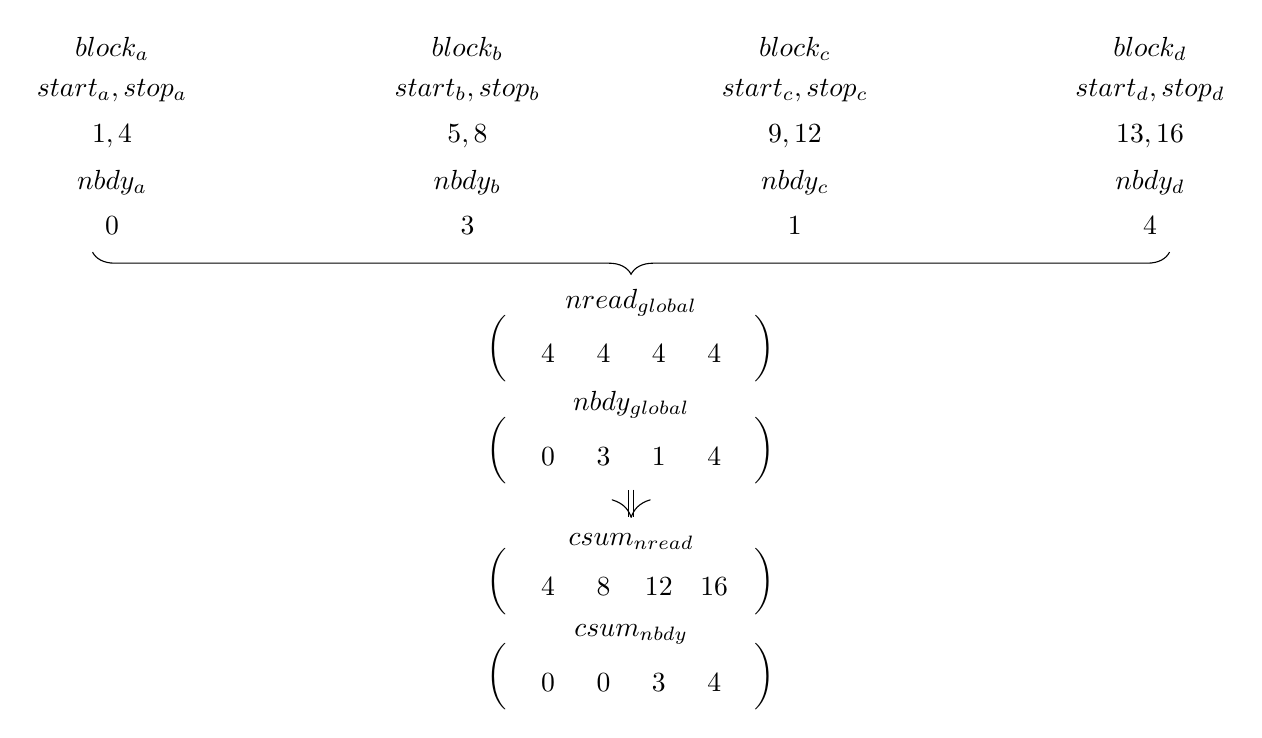
\begin{tikzpicture}[
    arr/.style={matrix of math nodes, left delimiter=(, right delimiter=), nodes={minimum width=2em}},
    smarr/.style={matrix of math nodes,
        % 1. Reduce space inside each cell (default is 0.333em)
        nodes={inner sep=1pt}, 
        % 2. Reduce space between rows and columns
        row sep=1pt,
        column sep=1pt,
        left delimiter=(, right delimiter=)},
    nopar/.style={matrix of math nodes, nodes={inner sep=1pt},row sep=1pt,column sep=1pt},
    map/.style={<->, shorten <=2pt, shorten >=2pt, thick},
    uni/.style={->},
    yield/.style={->,double,double equal sign distance,shorten <=2pt, shorten >=2pt},
    curly/.style={decorate,decoration={brace,amplitude=8pt,mirror,raise=4ex}}
]
    \node[below left=10mm and 60mm of current page.center] (anode) {$block_a$};
    \node[below left=10mm and 15mm of current page.center] (bnode) {$block_b$};
    \node[below right=10mm and 15mm of current page.center] (cnode) {$block_c$};
    \node[below right=10mm and 60mm of current page.center] (dnode) {$block_d$};
    
    \node[below=0mm] at (anode.south) (anums) {$start_a,stop_a$};
    \node[below=0mm] at (bnode.south) (bnums) {$start_b,stop_b$};
    \node[below=0mm] at (cnode.south) (cnums) {$start_c,stop_c$};
    \node[below=0mm] at (dnode.south) (dnums) {$start_d,stop_d$};
    
    \matrix (lista) [nopar, below=0mm of anums.south] {
        {1, 4} \\
    };
    \matrix (listb) [nopar, below=0mm of bnums.south] {
        {5, 8} \\
    };
    \matrix (listc) [nopar, below=0mm of cnums.south] {
        {9, 12} \\
    };
    \matrix (listd) [nopar, below=0mm of dnums.south] {
        {13, 16} \\
    };

    \node[below=0mm] at (lista.south) (nbdya) {$nbdy_a$};
    \node[below=0mm] at (listb.south) (nbdyb) {$nbdy_b$};
    \node[below=0mm] at (listc.south) (nbdyc) {$nbdy_c$};
    \node[below=0mm] at (listd.south) (nbdyd) {$nbdy_d$};
    
    \matrix (na) [nopar, below=0mm of nbdya.south] {
        0 \\
    };
    \matrix (nb) [nopar, below=0mm of nbdyb.south] {
        3 \\
    };
    \matrix (nc) [nopar, below=0mm of nbdyc.south] {
        1 \\
    };
    \matrix (nd) [nopar, below=0mm of nbdyd.south] {
        4 \\
    };

    \draw [curly] (na.north west) -- (nd.north east);

    \node[below=42mm of current page.center] (nread) {$nread_{global}$};
    \matrix (arrnread) [arr, below=0mm of nread.south] {
        4 & 4 & 4 & 4 \\
    };
    
    \node[below=0mm of arrnread.south] (nbdy) {$nbdy_{global}$};
    \matrix (arrnbdy) [arr, below=0mm of nbdy.south] {
        0 & 3 & 1 & 4 \\
    };

    \node[below=5mm of arrnbdy.south] (csumnread) {$csum_{nread}$};
    \matrix (arrcsumnread) [arr, below=0mm of csumnread.south] {
        4 & 8 & 12 & 16 \\
    };
    \node[below=0mm of arrcsumnread.south] (csumnbdy) {$csum_{nbdy}$};
    \matrix (arrcsumnbdy) [arr, below=0mm of csumnbdy.south] {
        0 & 0 & 3 & 4 \\
    };

    \draw[yield] (arrnbdy.south) -- (csumnread.north);
\end{tikzpicture}


\newpage
\subsubsection {Finding $nreqbyproc_{block}$, $reqindices_{block}$, and $nreqbyproc_{global}$}
First, reading in the $block$ assignments specific to a particular $block$ is required:
\\\\
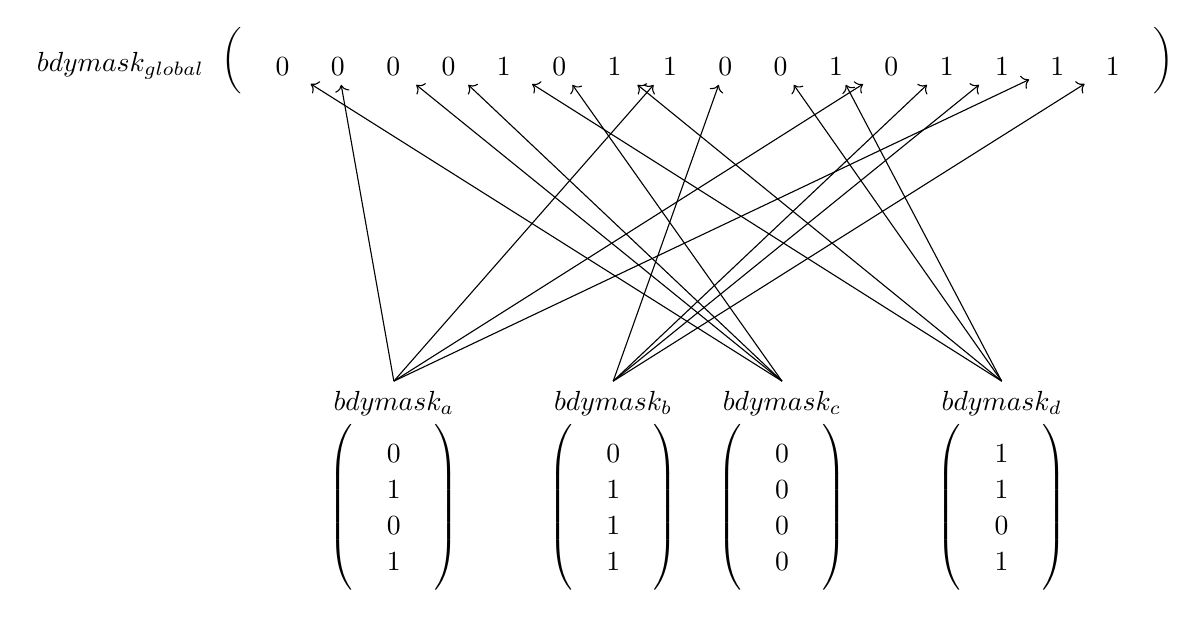
\begin{tikzpicture}[
    arr/.style={matrix of math nodes, left delimiter=(, right delimiter=), nodes={minimum width=2em}},
    map/.style={<->, shorten <=2pt, shorten >=2pt, thick},
    uni/.style={->}
]
    % Array C (shifted down)
    \matrix (C) [arr] {
    %   1   2   3   4   5   6   7   8   9  10  11  12  13  14  15  16
        0 & 0 & 0 & 0 & 1 & 0 & 1 & 1 & 0 & 0 & 1 & 0 & 1 & 1 & 1 & 1 \\
    };

    % Names
    \node[left=4mm of C] at (C.west) (cname) {$bdymask_{global}$} ;

    \node[below right=40mm and 10mm of C] at (C.west) (anode) {$bdymask_a$};
    \node[below right=40mm and 38mm of C] at (C.west) (bnode) {$bdymask_b$};
    \node[below left=40mm and 38mm of C] at (C.east) (cnode) {$bdymask_c$};
    \node[below left=40mm and 10mm of C] at (C.east) (dnode) {$bdymask_d$};

    
    \draw[uni] (anode.north) -- (C-1-2);
    \draw[uni] (anode.north) -- (C-1-8);
    \draw[uni] (anode.north) -- (C-1-12);
    \draw[uni] (anode.north) -- (C-1-15);
    
    \draw[uni] (bnode.north) -- (C-1-9);
    \draw[uni] (bnode.north) -- (C-1-13);
    \draw[uni] (bnode.north) -- (C-1-14);
    \draw[uni] (bnode.north) -- (C-1-16);
    
    \draw[uni] (cnode.north) -- (C-1-1);
    \draw[uni] (cnode.north) -- (C-1-3);
    \draw[uni] (cnode.north) -- (C-1-4);
    \draw[uni] (cnode.north) -- (C-1-6);

    \draw[uni] (dnode.north) -- (C-1-5);
    \draw[uni] (dnode.north) -- (C-1-7);
    \draw[uni] (dnode.north) -- (C-1-10);
    \draw[uni] (dnode.north) -- (C-1-11);

    \matrix (arra) [arr, below=0mm of anode.south] {
        0 \\ 1 \\ 0 \\ 1 \\
    };
    \matrix (arrb) [arr, below=0mm of bnode.south] {
        0 \\ 1 \\ 1 \\ 1 \\
    };
    \matrix (arrc) [arr, below=0mm of cnode.south] {
        0 \\ 0 \\ 0 \\ 0 \\
    };
    \matrix (arrd) [arr, below=0mm of dnode.south] {
        1 \\1 \\ 0 \\ 1 \\
    };
\end{tikzpicture}
\\\\
Next, each $block$ loops over its assignments, and if $bdymask_{*_i} > 0$ then record
information about $indices_{block}[i]$ in $pth$ index of process arrays
$nreqbyproc_{block}$ and $reqindices_{block}$. Note that in $reqindices_{block}$
the first subscript is equal to $ith$ index mapping to $indices_{block}$ and the
second subscript is equal to $jth$ occurrence of $bdymask_{*_i} > 0$. Examining $block_a$:
\\\\
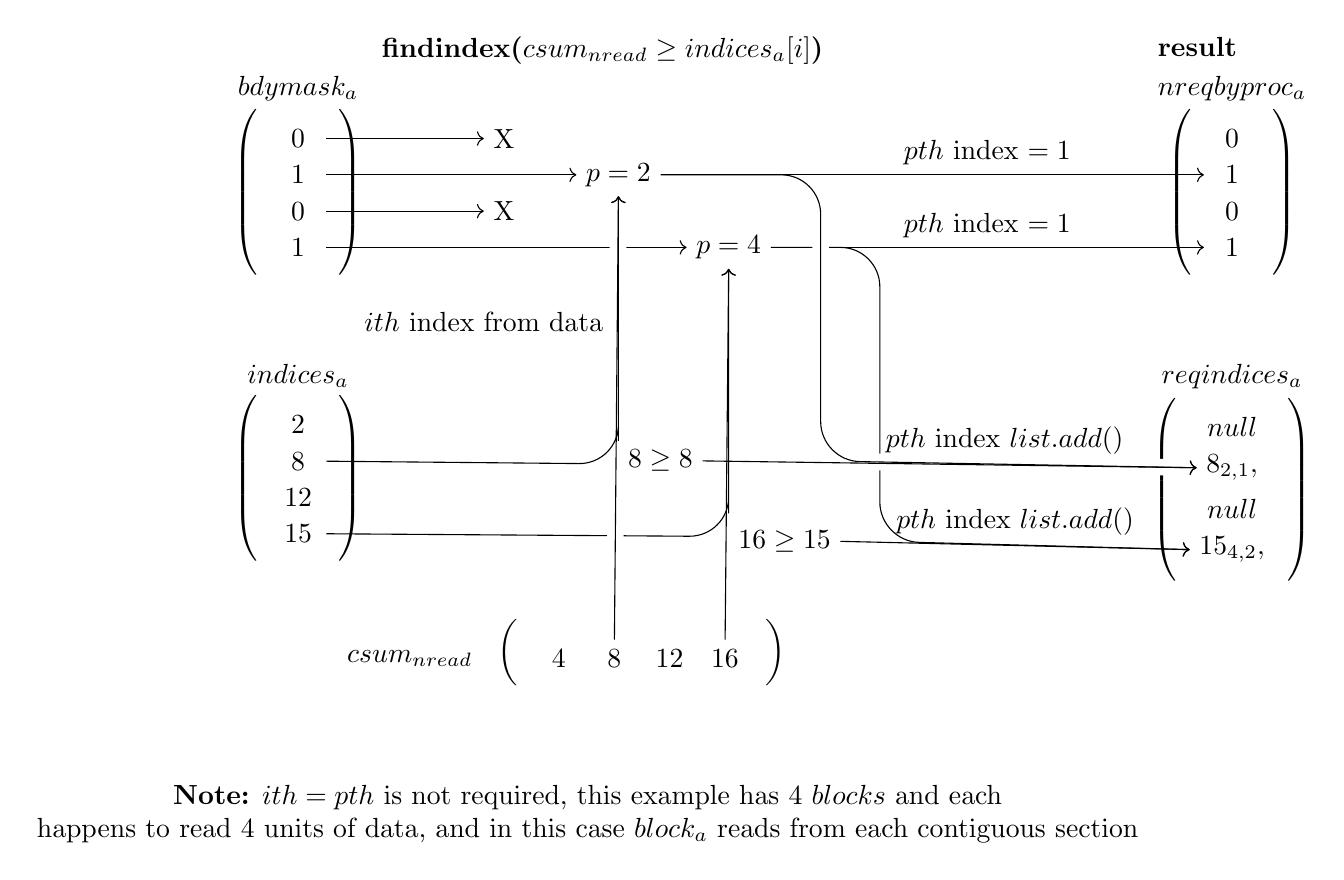
\begin{tikzpicture}[
    arr/.style={matrix of math nodes, left delimiter=(, right delimiter=), nodes={minimum width=2em}},
    map/.style={<->, shorten <=2pt, shorten >=2pt, thick},
    uni/.style={->},
    round/.style={->,rounded corners=5mm}
]
    \node[below=10mm of current page.west] (anode) {$bdymask_a$};
    \matrix (arra) [arr, below=0mm of anode.south] {
        0 \\ 1 \\ 0 \\ 1 \\
    };
    \node[below=10mm of arra.south] (bnode) {$indices_a$};
    \matrix (arrb) [arr, below=0mm of bnode.south] {
        2 \\ 8 \\ 12 \\ 15 \\
    };
    \node[below right=10mm and 5mm of arrb.south] (csumnode) {$csum_{nread}$};
    \matrix (arrcsum) [arr, right=5mm of csumnode.east] {
        4 & 8 & 12 & 16 \\
    };

    \node[below left=5mm and 40mm of current page.center] (findcsum) {\textbf{findindex($csum_{nread} \ge indices_a[i]$)}};
    \node[below left=40mm and 68mm of current page.center] (noteith) {$ith$ index from data};

    \node[right=20mm of arra-1-1.east] (noop1) {X};
    \node[right=20mm of arra-3-1.east] (noop2) {X};
    \draw[uni] (arra-1-1.east) -- (noop1.west);
    \draw[uni] (arra-3-1.east) -- (noop2.west);

    
    \node[right=31.75mm of arra-2-1.east] (op1) {$p=2$};
    \draw[uni] (arra-2-1.east) -- (op1.west);

    \node[right=45.75mm of arra-4-1.east] (op2) {$p=4$};    
    \draw[uni] (arra-4-1.east) -- (op2.west);

    % draw op2 first to show op1 on top with white out line
    \draw[round] (arrb-4-1.east) -- ([yshift=-34mm]op2.south) -| (op2.south);
    \draw[uni] (arrcsum-1-4) -- (op2.south);

    \draw[uni,preaction={draw=white,-,line width=6pt}] (arrcsum-1-2) -- (op1.south);
    \draw[round] (arrb-2-1.east) -- ([yshift=-34mm]op1.south) -| (op1.south);

    \node[below right=31mm and 0mm of op1.south] (pmathop1) {$8 \ge 8$};
    \node[below right=32mm and 0mm of op2.south] (pmathop2) {$16 \ge 15$};

    % resulting output
    \node[below right=5mm and 0mm of current page.center] (result) {\textbf{result}};
    \node[below right=10mm and 0mm of current page.center] (nreqbyproc) {$nreqbyproc_a$};
    \matrix (arrnproc) [arr, below=0mm of nreqbyproc.south] {
        0 \\ 1 \\ 0 \\ 1 \\
    };
    \node[below=10mm of arrnproc.south] (reqind) {$reqindices_a$};
    \matrix (arrind) [arr, below=0mm of reqind.south] {
        {null} \\ {8_{2,1},} \\ {null} \\ {15_{4,2},} \\
    };
    
    % draw op2 first to show op1 on top with white out line
    \draw[round] (op2.east) -| ([xshift=5mm]pmathop2.east) -- (arrind-4-1.west);
    \draw[uni] (pmathop2.east) -- (arrind-4-1.west) node[midway,above] (listval2) {$pth$ index $list.add()$};;
    \draw[uni] (op2.east) -- (arrnproc-4-1.west) node[midway,above] (procval2) {$pth$ index $=1$};
    
    \draw[round,preaction={draw=white,-,line width=6pt}] (op1.east) -| ([xshift=15mm]pmathop1.east) -- (arrind-2-1.west);
    \draw[uni] (pmathop1.east) -- (arrind-2-1.west) node[midway,above,xshift=7mm] (listval1) {$pth$ index $list.add()$};
    \draw[uni] (op1.east) -- (arrnproc-2-1.west) node[midway,above,xshift=7mm] (procval1) {$pth$ index $=1$};

    \node[below left=100mm and 0mm of current page.center,align=center]
            {\textbf{Note:} $ith = pth$ is not required, this example has $4$ $blocks$ and each \\
            happens to read $4$ units of data, and in this case $block_a$ reads from each contiguous section} ;
\end{tikzpicture}
\newpage
If done for each $block$, the results should yield:
\\\\

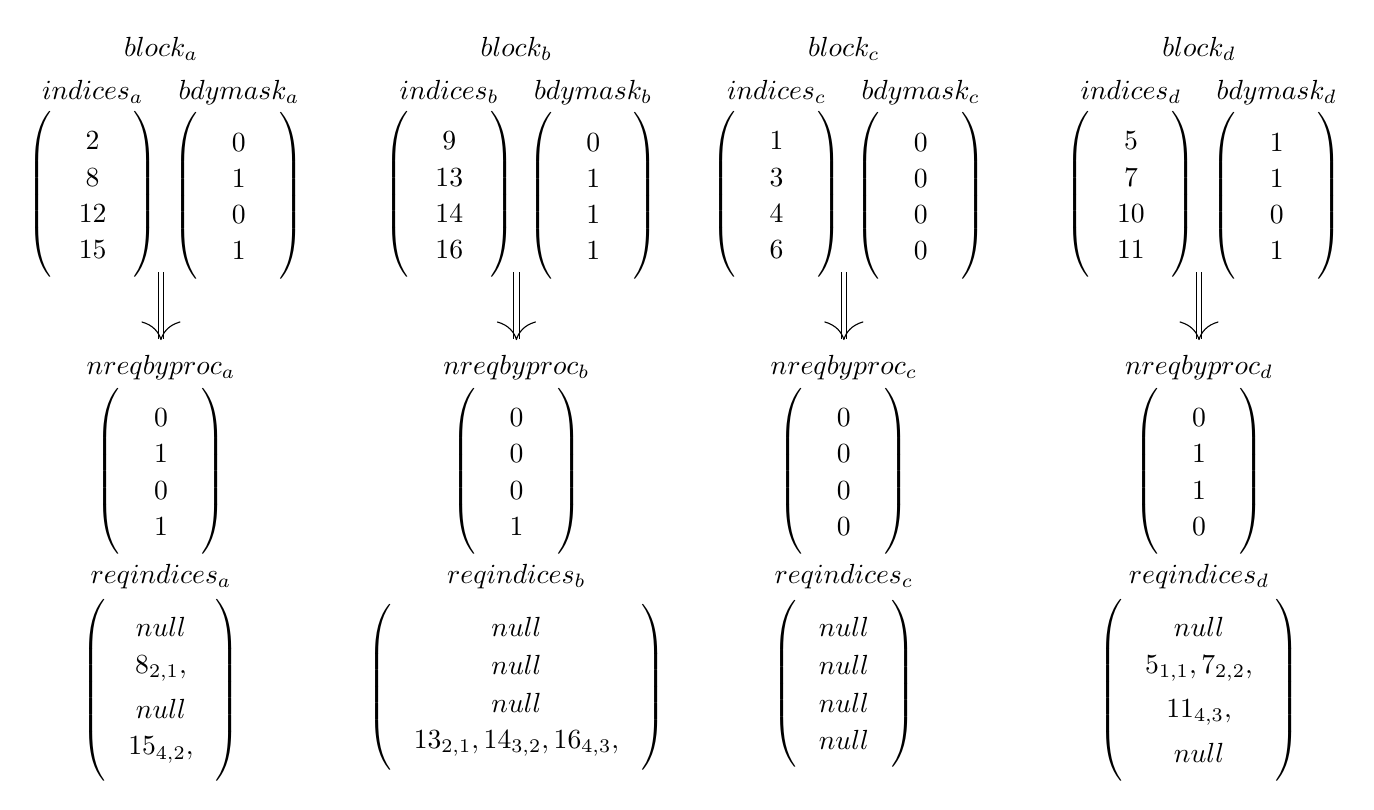
\begin{tikzpicture}[
    arr/.style={matrix of math nodes, left delimiter=(, right delimiter=), nodes={minimum width=2em}},
    smarr/.style={matrix of math nodes,
        % 1. Reduce space inside each cell (default is 0.333em)
        nodes={inner sep=1pt}, 
        % 2. Reduce space between rows and columns
        row sep=1pt,
        column sep=1pt,
        left delimiter=(, right delimiter=)},
    nopar/.style={matrix of math nodes, nodes={inner sep=1pt},row sep=1pt,column sep=1pt},
    map/.style={<->, shorten <=2pt, shorten >=2pt, thick},
    uni/.style={->},
    yield/.style={->,double,double equal sign distance,shorten <=2pt, shorten >=2pt},
    curly/.style={decorate,decoration={brace,amplitude=8pt,mirror,raise=4ex}}
]
    \node[below left=10mm and 60mm of current page.center] (ablock) {$block_a$};
    \node[below left=10mm and 15mm of current page.center] (bblock) {$block_b$};
    \node[below right=10mm and 15mm of current page.center] (cblock) {$block_c$};
    \node[below right=10mm and 60mm of current page.center] (dblock) {$block_d$};



    \node[below left=0mm and 1mm of ablock.south] (aind) {$indices_a$};
    \node[below left=0mm and 1mm of bblock.south] (bind) {$indices_b$};
    \node[below left=0mm and 1mm of cblock.south] (cind) {$indices_c$};
    \node[below left=0mm and 1mm of dblock.south] (dind) {$indices_d$};
    \matrix (arridxa) [arr, below=0mm of aind.south] {
        2 \\ 8 \\ 12 \\ 15 \\
    };
    \matrix (arridxb) [arr, below=0mm of bind.south] {
        9 \\ 13 \\ 14 \\ 16 \\
    };
    \matrix (arridxc) [arr, below=0mm of cind.south] {
        1 \\ 3 \\ 4 \\ 6 \\
    };
    \matrix (arridxd) [arr, below=0mm of dind.south] {
        5 \\ 7 \\ 10 \\ 11 \\
    };

    \node[below right=0mm and 1mm of ablock.south] (abdy) {$bdymask_a$};
    \node[below right=0mm and 1mm of bblock.south] (bbdy) {$bdymask_b$};
    \node[below right=0mm and 1mm of cblock.south] (cbdy) {$bdymask_c$};
    \node[below right=0mm and 1mm of dblock.south] (dbdy) {$bdymask_d$};
    \matrix (arrbdya) [arr, below=0mm of abdy.south] {
        0 \\ 1 \\ 0 \\ 1 \\
    };
    \matrix (arrbdyb) [arr, below=0mm of bbdy.south] {
        0 \\ 1 \\ 1 \\ 1 \\
    };
    \matrix (arrbdyc) [arr, below=0mm of cbdy.south] {
        0 \\ 0 \\ 0 \\ 0 \\
    };
    \matrix (arrbdyd) [arr, below=0mm of dbdy.south] {
        1 \\1 \\ 0 \\ 1 \\
    };

    
    \node[below=35mm] at (ablock.south) (anums) {$nreqbyproc_a$};
    \node[below=35mm] at (bblock.south) (bnums) {$nreqbyproc_b$};
    \node[below=35mm] at (cblock.south) (cnums) {$nreqbyproc_c$};
    \node[below=35mm] at (dblock.south) (dnums) {$nreqbyproc_d$};
    
    \matrix (nreqa) [arr, below=0mm of anums.south] {
        0 \\ 1 \\ 0 \\ 1 \\
    };
    \matrix (nreqb) [arr, below=0mm of bnums.south] {
        0 \\ 0 \\ 0 \\ 1 \\
    };
    \matrix (nreqc) [arr, below=0mm of cnums.south] {
        0 \\ 0 \\ 0 \\ 0 \\
    };
    \matrix (nreqd) [arr, below=0mm of dnums.south] {
        0 \\ 1 \\ 1 \\ 0 \\
    };

    \node[below=0mm] at (nreqa.south) (areqind) {$reqindices_a$};
    \node[below=0mm] at (nreqb.south) (breqind) {$reqindices_b$};
    \node[below=0mm] at (nreqc.south) (creqind) {$reqindices_c$};
    \node[below=0mm] at (nreqd.south) (dreqind) {$reqindices_d$};
    
    \matrix (reqinda) [arr, below=0mm of areqind.south] {
        {null} \\ {8_{2,1},} \\ {null} \\ {15_{4,2},} \\
    };
    \matrix (reqindb) [arr, below=0mm of breqind.south] {
        {null} \\ {null} \\ {null} \\ {13_{2,1},14_{3,2},16_{4,3},} \\
    };
    \matrix (reqindc) [arr, below=0mm of creqind.south] {
        {null} \\ {null} \\ {null} \\ {null} \\
    };
    \matrix (reqindd) [arr, below=0mm of dreqind.south] {
        {null} \\ {5_{1,1},7_{2,2},} \\ {11_{4,3},} \\ {null} \\
    };


    \draw[yield] ([yshift=10mm]anums.north) -- (anums.north);
    \draw[yield] ([yshift=10mm]bnums.north) -- (bnums.north);
    \draw[yield] ([yshift=10mm]cnums.north) -- (cnums.north);
    \draw[yield] ([yshift=10mm]dnums.north) -- (dnums.north);
\end{tikzpicture}
\\\\
Finding $nreqbyproc_{global}$ is performed by index-wise summation of each $nreqbyproc_*$:
\\\\

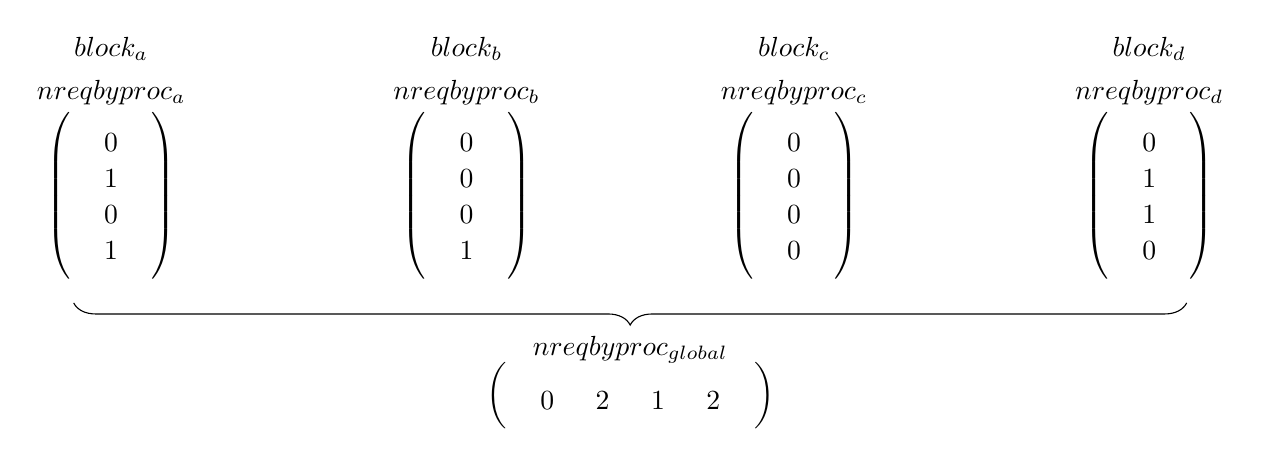
\begin{tikzpicture}[
    arr/.style={matrix of math nodes, left delimiter=(, right delimiter=), nodes={minimum width=2em}},
    smarr/.style={matrix of math nodes,
        % 1. Reduce space inside each cell (default is 0.333em)
        nodes={inner sep=1pt}, 
        % 2. Reduce space between rows and columns
        row sep=1pt,
        column sep=1pt,
        left delimiter=(, right delimiter=)},
    nopar/.style={matrix of math nodes, nodes={inner sep=1pt},row sep=1pt,column sep=1pt},
    map/.style={<->, shorten <=2pt, shorten >=2pt, thick},
    uni/.style={->},
    yield/.style={->,double,double equal sign distance,shorten <=2pt, shorten >=2pt},
    curly/.style={decorate,decoration={brace,amplitude=8pt,mirror,raise=4ex}}
]
    \node[below left=10mm and 60mm of current page.center] (anode) {$block_a$};
    \node[below left=10mm and 15mm of current page.center] (bnode) {$block_b$};
    \node[below right=10mm and 15mm of current page.center] (cnode) {$block_c$};
    \node[below right=10mm and 60mm of current page.center] (dnode) {$block_d$};
    
    \node[below=0mm] at (anode.south) (anums) {$nreqbyproc_a$};
    \node[below=0mm] at (bnode.south) (bnums) {$nreqbyproc_b$};
    \node[below=0mm] at (cnode.south) (cnums) {$nreqbyproc_c$};
    \node[below=0mm] at (dnode.south) (dnums) {$nreqbyproc_d$};
    
    \matrix (nreqa) [arr, below=0mm of anums.south] {
        0 \\ 1 \\ 0 \\ 1 \\
    };
    \matrix (nreqb) [arr, below=0mm of bnums.south] {
        0 \\ 0 \\ 0 \\ 1 \\
    };
    \matrix (nreqc) [arr, below=0mm of cnums.south] {
        0 \\ 0 \\ 0 \\ 0 \\
    };
    \matrix (nreqd) [arr, below=0mm of dnums.south] {
        0 \\ 1 \\ 1 \\ 0 \\
    };
    
    \draw [curly] ([yshift=3mm]nreqa.south west) -- ([yshift=3mm]nreqd.south east);

    \node[below=48mm of current page.center] (nreq) {$nreqbyproc_{global}$};
    \matrix (arrnreq) [arr, below=0mm of nreq.south] {
        0 & 2 & 1 & 2 \\
    };
\end{tikzpicture}
\newpage
\subsubsection {Communication Loops}
The $nreqbyproc_{global}$ corresponds to how many in degrees each $block$ will have
when communicating the contiguous chunks to the specific $block$ assignments (if
the $block$ also communicates to itself). Each $block$ sends the $ids$ (from $reqindices_{block}$)
it needs to the $block$ that read it in, which then responds with the analogous $bdy_*$
value for those $ids$.
\\\\
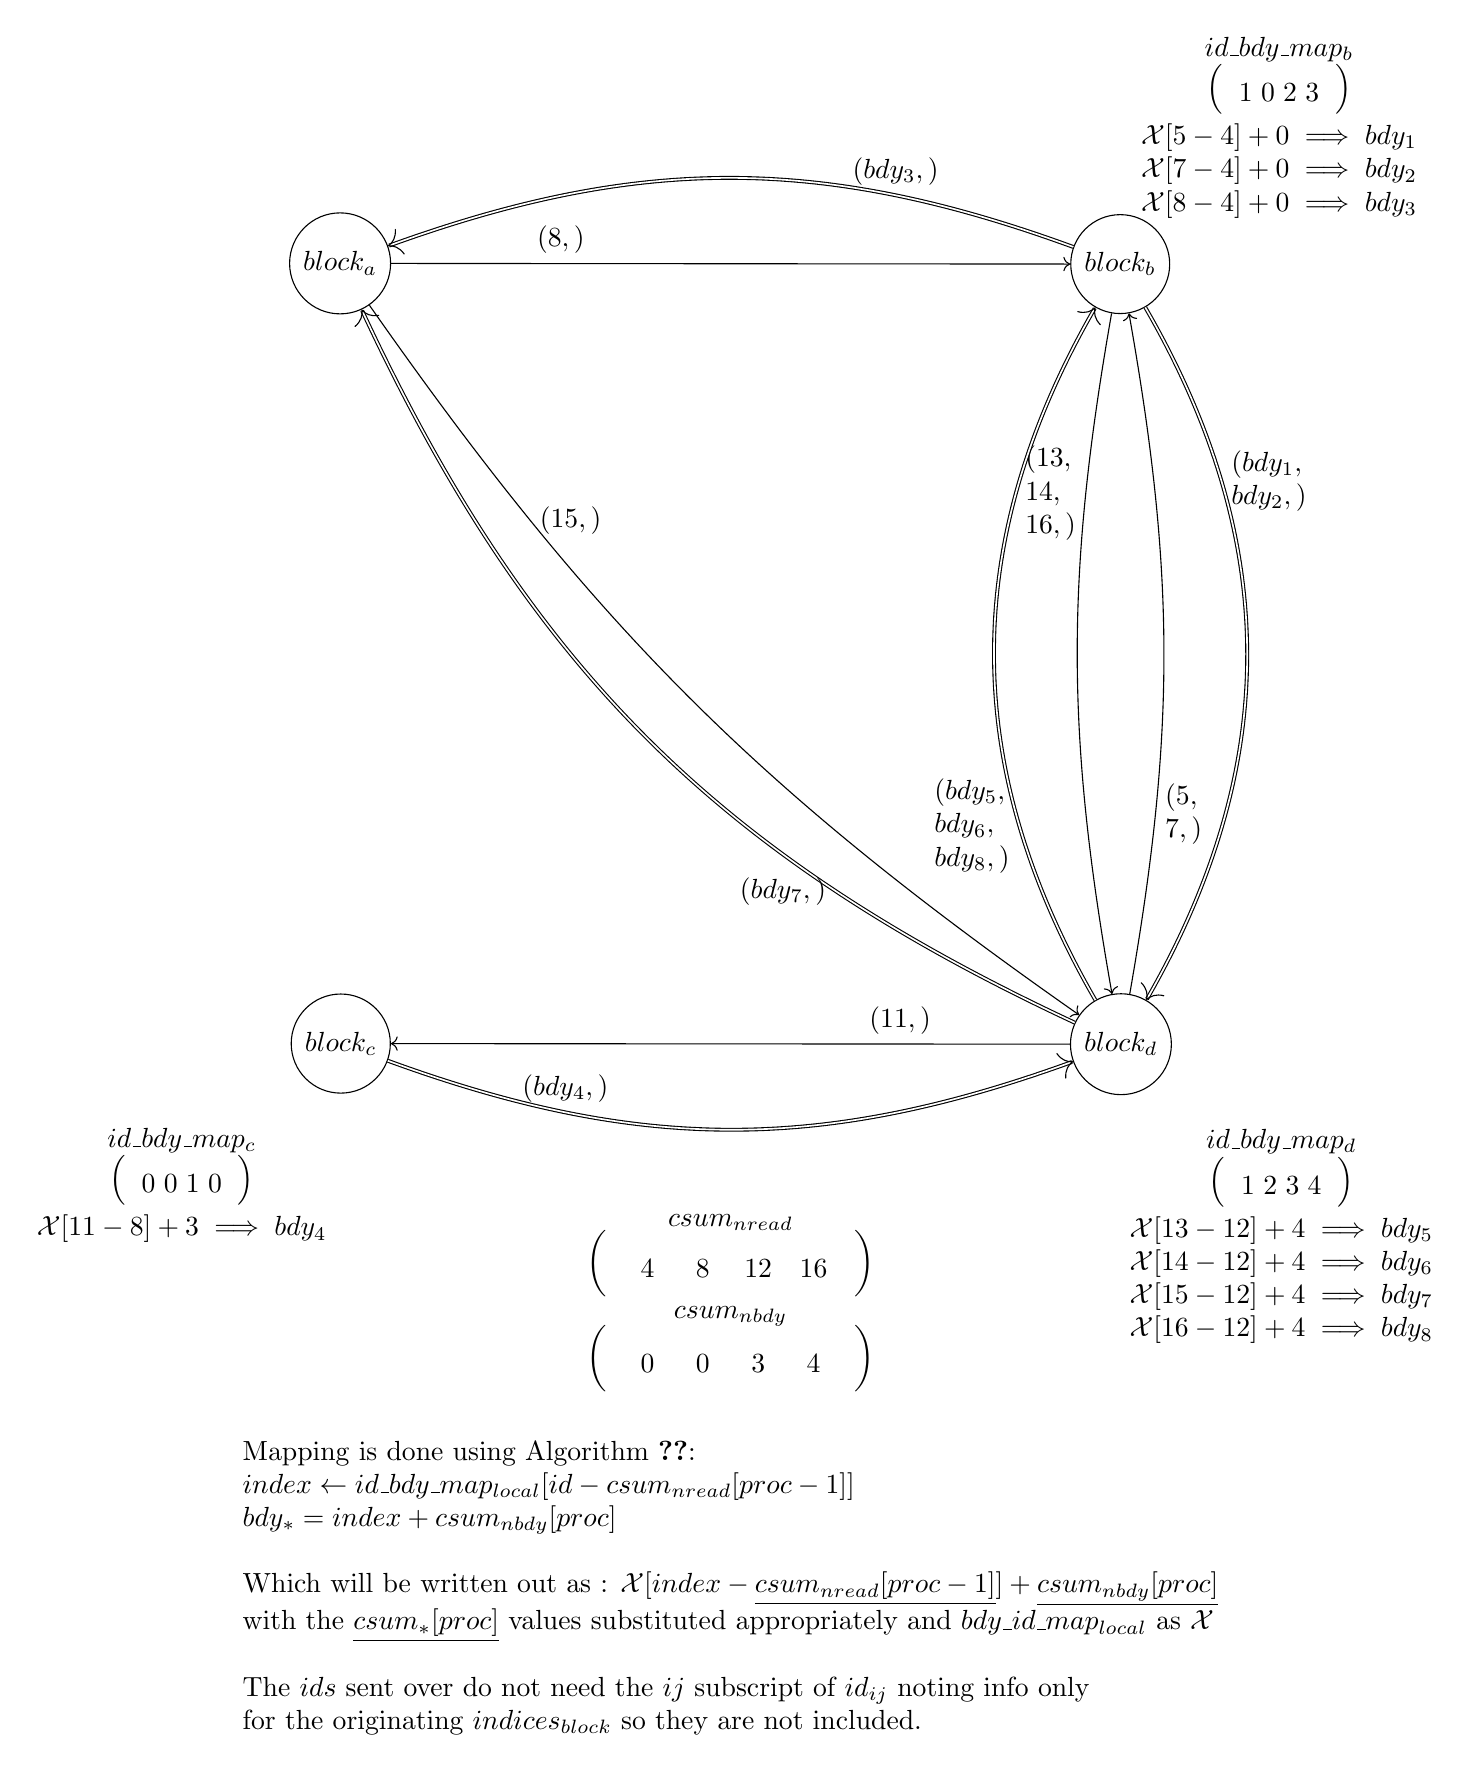
\begin{tikzpicture}[
    arr/.style={matrix of math nodes, left delimiter=(, right delimiter=), nodes={minimum width=2em}},
    smarr/.style={matrix of math nodes,
        % 1. Reduce space inside each cell (default is 0.333em)
        nodes={inner sep=1pt}, 
        % 2. Reduce space between rows and columns
        row sep=1pt,
        column sep=1pt,
        left delimiter=(, right delimiter=)},
    nopar/.style={matrix of math nodes, nodes={inner sep=1pt},row sep=1pt,column sep=1pt},
    map/.style={<->, shorten <=2pt, shorten >=2pt, thick},
    uni/.style={->},
    yield/.style={->,double,double equal sign distance,shorten <=2pt, shorten >=2pt},
    curly/.style={decorate,decoration={brace,amplitude=8pt,mirror,raise=4ex}}
]
    \node[draw, circle, above left =45mm and 45mm of current page.center] (anode) {$block_a$};
    \node[draw, circle, above right=45mm and 45mm of current page.center] (bnode) {$block_b$};
    \node[draw, circle, below left =45mm and 45mm of current page.center] (cnode) {$block_c$};
    \node[draw, circle, below right=45mm and 45mm of current page.center] (dnode) {$block_d$};

    % Inbound Indices Request
    \draw (anode) edge[->] node[above,near start] () {$(8,)$} (bnode);
    \draw (anode) edge[->, bend right=10] node[right,near start] () {$(15,)$} (dnode);
    
    \draw (bnode) edge[->, bend right=10] node[left,near start, align=left] () {$(13,$\\$14,$\\$16,)$} (dnode);

    % None
    % \draw (cnode) edge[->] node[above,near start] () {$(8,)$} (bnode);
    
    \draw (dnode) edge[->, bend right=10] node[right,near start, align=left] () {$(5,$\\$7,)$} (bnode);
    \draw (dnode) edge[->] node[above,near start] () {$(11,)$} (cnode);


    % Outbound Bdy Response
    \draw (bnode) edge[->,double, bend right=20] node[above,near start] () {$(bdy_3,)$} (anode);
    \draw (dnode) edge[->,double, bend left=20] node[left,near start] () {$(bdy_7,)$} (anode);
    
    \draw (dnode) edge[->, double, bend left=30] node[left,near start,align=left] () {$(bdy_5,$\\$bdy_6,$\\$bdy_8,)$} (bnode);

    % % None
    % % \draw (cnode) edge[->] node[above,near start] () {$(8,)$} (bnode);
    
    \draw (bnode) edge[->, double, bend left=30] node[right,near start, align=left] () {$(bdy_1,$\\$bdy_2,)$} (dnode);
    \draw (cnode) edge[->, double, bend right=20] node[above,near start] () {$(bdy_4,)$} (dnode);
    
    \node[above right=20mm and 5mm of bnode, align=left] (bbdyid) {$id\_bdy\_map_b$};
    \node[below left =5mm and 5mm of cnode, align=left] (cbdyid) {$id\_bdy\_map_c$};
    \node[below right=5mm and 5mm of dnode, align=left] (dbdyid) {$id\_bdy\_map_d$};

    \matrix (arridb) [smarr, below=0mm of bbdyid.south] {
        1 & 0 & 2 & 3 \\
    };
    \matrix (arridc) [smarr, below=0mm of cbdyid.south] {
        0 & 0 & 1 & 0 \\
    };
    \matrix (arridd) [smarr, below=0mm of dbdyid.south] {
        1 & 2 & 3 & 4 \\
    };

    \node[below=0mm of arridb.south, align=left] ()
        {
            $\mathcal{X}[5 - 4] + 0 \implies bdy_1$\\
            $\mathcal{X}[7 - 4] + 0 \implies bdy_2$\\
            $\mathcal{X}[8 - 4] + 0 \implies bdy_3$\\
        };
    
    \node[below=0mm of arridc.south, align=left] ()
        {
            $\mathcal{X}[11 - 8] + 3 \implies bdy_4$\\
        };
    
    \node[below=0mm of arridd.south, align=left] ()
        {
            $\mathcal{X}[13 - 12] + 4 \implies bdy_5$\\
            $\mathcal{X}[14 - 12] + 4 \implies bdy_6$\\
            $\mathcal{X}[15 - 12] + 4 \implies bdy_7$\\
            $\mathcal{X}[16 - 12] + 4 \implies bdy_8$\\
        };

    \node[below=70mm of current page.center] (csumnread) {$csum_{nread}$};
    \matrix (arrcsumnread) [arr, below=0mm of csumnread.south] {
        4 & 8 & 12 & 16 \\
    };
    \node[below=0mm of arrcsumnread.south] (csumnbdy) {$csum_{nbdy}$};
    \matrix (arrcsumnbdy) [arr, below=0mm of csumnbdy.south] {
        0 & 0 & 3 & 4 \\
    };

    \node[below=5mm of arrcsumnbdy, align=left] () {
        Mapping is done using Algorithm~\ref{decomp}:\\
        $index \gets id\_bdy\_map_{local}[id - csum_{nread}[proc-1]]$\\
        $bdy_*= index+csum_{nbdy}[proc]$\\
        \\
        Which will be written out as : 
        $\mathcal{X}[index-\underline{csum_{nread}[proc-1]}] + \underline{csum_{nbdy}[proc]}$\\
        with the $\underline{csum_*[proc]}$ values substituted appropriately 
        and $bdy\_id\_map_{local}$ as $\mathcal{X}$\\
        \\
        The $ids$ sent over do not need the $ij$ subscript of $id_{ij}$ noting info only\\
        for the originating $indices_{block}$ so they are not included.
        };
    
\end{tikzpicture}
\newpage
\subsubsection {Final Assignment}
As each respective $block$ receives the corresponding $bdy_*$ value to each $id_{ij}$,
the construction of the $id\_bdy\_map_{block}$, $bdy\_id\_map_{block}$, and set of
owned $bdy_*$ can be done.\\
\\
The method shown in Algorithm~\ref{decomp} implies a linear processing, but this
is not strictly necessary as each set of communicated values is self sufficient
and can be processed independently.\\
\\
As before, $block_a$ will be used first as an example:
\\\\
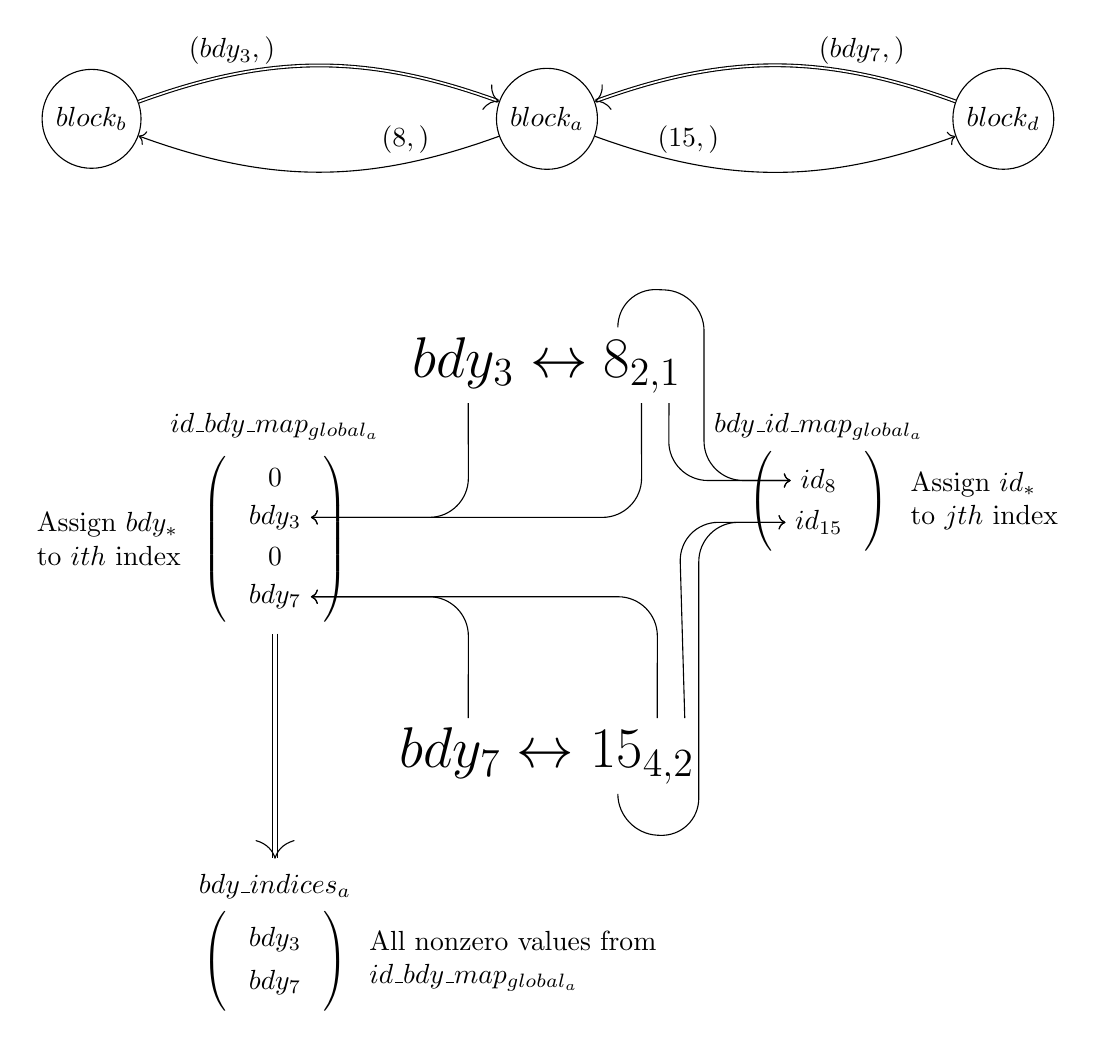
\begin{tikzpicture}[
    arr/.style={matrix of math nodes, left delimiter=(, right delimiter=), nodes={minimum width=2em}},
    smarr/.style={matrix of math nodes,
        % 1. Reduce space inside each cell (default is 0.333em)
        nodes={inner sep=1pt}, 
        % 2. Reduce space between rows and columns
        row sep=1pt,
        column sep=1pt,
        left delimiter=(, right delimiter=)},
    round/.style={->,rounded corners=5mm},
    nopar/.style={matrix of math nodes, nodes={inner sep=1pt},row sep=1pt,column sep=1pt},
    map/.style={<->, shorten <=2pt, shorten >=2pt, thick},
    uni/.style={->},
    yield/.style={->,double,double equal sign distance,shorten <=2pt, shorten >=2pt},
    curly/.style={decorate,decoration={brace,amplitude=8pt,mirror,raise=4ex}}
]
    \node[draw, circle, above right=5mm and 65mm of current page.center,xshift=20mm] (anode) {$block_a$};

    \node[draw, circle, left=45mm of anode] (bnode) {$block_b$};
    \node[draw, circle, right=45mm of anode] (dnode) {$block_d$};

    % Inbound Indices Request
    \draw (anode) edge[->, bend left=20] node[above,near start] () {$(8,)$} (bnode);
    \draw (anode) edge[->, bend right=20] node[above,near start] () {$(15,)$} (dnode);

    % Outbound Bdy Response
    \draw (bnode) edge[->,double, bend left=20] node[above,near start] () {$(bdy_3,)$} (anode);
    \draw (dnode) edge[->,double, bend right=20] node[above,near start] () {$(bdy_7,)$} (anode);


    \node [below=20mm of anode.south,font=\huge] (first) {$bdy_3 \leftrightarrow 8_{2,1}$};
    \node [below=40mm of first.south,font=\huge] (second) {$bdy_7 \leftrightarrow 15_{4,2}$};


    \node [below left=0mm and 20mm of first.south] (idbdy_global) {$id\_bdy\_map_{global_a}$};
    \matrix (arridbdy_global) [arr, below=0mm of idbdy_global.south] {
        0 \\ bdy_3 \\ 0 \\ bdy_7 \\
    };

    \node [below right=0mm and 20mm of first.south] (bdyid_global) {$bdy\_id\_map_{global_a}$};
    \matrix (arrbdyid_global) [arr, below=0mm of bdyid_global.south] {
        id_{8} \\ id_{15} \\
    };

    % left map of data to id_bdy_map
    \draw[round] ([xshift=-10mm]first.south) -- ([xshift=20mm]arridbdy_global-2-1.east) -- (arridbdy_global-2-1.east);
    \draw[round] ([xshift=12mm]first.south) -- ([xshift=42mm]arridbdy_global-2-1.east) -- (arridbdy_global-2-1.east);

    \draw[round] ([xshift=-10mm]second.north) -- ([xshift=20mm]arridbdy_global-4-1.east) -- (arridbdy_global-4-1.east);
    \draw[round] ([xshift=14mm]second.north) -- ([xshift=44mm]arridbdy_global-4-1.east) -- (arridbdy_global-4-1.east);

    % right map of data to bdy_id_map
    \draw[round] ([xshift=9mm]first.north)
              -- ([xshift=9mm,yshift=5mm]first.north)
              -- ([xshift=-11mm,yshift=24mm]arrbdyid_global-1-1.west)
              -- ([xshift=-11mm]arrbdyid_global-1-1.west)
              -- (arrbdyid_global-1-1.west);  
    \draw[round] ([xshift=15.5mm]first.south) -- ([xshift=-15.5mm]arrbdyid_global-1-1.west) -- (arrbdyid_global-1-1.west);

    \draw[round] ([xshift=9mm]second.south)
              -- ([xshift=9mm,yshift=-5mm]second.south)
              -- ([xshift=-11mm,yshift=-40mm]arrbdyid_global-2-1.west)
              -- ([xshift=-11mm]arrbdyid_global-2-1.west)
              -- (arrbdyid_global-2-1.west);  
    \draw[round] ([xshift=17.5mm]second.north) -- ([xshift=-13.5mm]arrbdyid_global-2-1.west) -- (arrbdyid_global-2-1.west);

    \node [align=left, left=5mm of arridbdy_global.west] (notea) {Assign $bdy_*$\\to $ith$ index};
    \node [align=left, right=5mm of arrbdyid_global.east] (noteb) {Assign $id_*$\\to $jth$ index};

    \node [below=30mm of arridbdy_global.south] (bdyindices) {$bdy\_indices_a$};
    \matrix (arrbdy) [arr, below=0mm of bdyindices.south] {
        bdy_3 \\ bdy_7 \\
    };
    \draw[yield] (arridbdy_global.south) -- (bdyindices.north);
    \node [align=left, right=5mm of arrbdy.east] (notec) {All nonzero values from\\$id\_bdy\_map_{global_a}$};

\end{tikzpicture}
\end{document}